\section*{Problem 3: 90 \degree Hybrid Junction with Tee}
\addcontentsline{toc}{section}{Problem 3: 90 \degree Hybrid Junction with Tee}

\subsection*{Problem 3a: Deriving Some Result}
\addcontentsline{toc}{subsection}{Problem 3a: Deriving Some Result}

This problem was pretty fun to solve. The first thing to realize is that the
system is matched everywhere (despite the potential difference in the transmission line
lengths at the tee). The impedance looking into just the tee (not cascaded with
the hybrid junction) is $\frac{\left( Z_0/\sqrt{2} \right)^2}{Z_{L}}$, where
$Z_L$ is the equivalent impedance of the two branches in the tee ($Z_L =
\frac{Z_0}{2}$). This means the input impedance to the tee is $Z_0$. The 90
\degree hybrid junction is matched by design. Thus, the cascade of these two
devices is matched. Now, the hybrid tee will propagate some input voltage
$V_{in}$ in the following way: At the end of one end of the branch (the one of
length a) the following voltage will appear:

\[ 
    V_a = \frac{V_{in}}{2} e^{-j \beta a} 
\]

At the end of the other branch (of length b-a) will appear the other voltage:

\[ 
    V_{b-a} = \frac{V_{in}}{2} e^{-j \beta \left( b-a \right)} 
\]

Now, the voltage appearing at port 2 because of the voltages at ports 1 and 4
($V_{b-a}$ and $V_a$, respectively) is:

\[ 
    V_2 = \frac{-1}{\sqrt{2}} \left( j V_a + V_{b-a}  \right) 
\]

Similarly, the voltage appearing at port 3 because of the voltages at ports 1
and 4 is:

\[ 
    V_3 = \frac{-1}{\sqrt{2}} \left( j V_{b-a} +  V_{a} \right)
\]

This can be seen by inspecting the scattering parameters of the 90 \degree
hybrid coupler:

\[ 
    S_{90\degree} = -\frac{j}{\sqrt{2}} \begin{pmatrix}
        0 & 1 & -j & 0 \\ 1 & 0 & 0 & -j \\ -j & 0 & 0 & 1 \\ 0 & -j & 1 & 0
    \end{pmatrix} 
\]

Now, the power coming out of port 2 is $\frac{|V_2|^2}{Z_0}$ and similarly with
the port coming out of port 3. Thus:

\[ 
    \frac{P_3}{P_2} = \frac{\left| V_3 \right|^2}{\left| V_2 \right|^2} 
\]

The prefactors in front of $V_2$ and $V_3$ can evidently be dropped (since they
are the same). This leaves the following expression to be evaluated:

\[
    \frac{P_3}{P_2} = \frac{\left| jV_{b-a} + V_a \right|^2}{\left| j V_a +
    V_{b-a} \right|^2} = \frac{\left| V_a \right|^2 + \left| V_{b-a} \right|^2 +
    jV_{b-a} V_a^* - j V_{b-a}^*V_a }{\left| V_a \right|^2 + \left| V_{b-a} \right|^2 +
j V_a V_{b-a}^* -j V_a^* V_{b-a}}
\]

But, $\left| V_a \right| = \left| V_{b-a} \right| = \frac{V_{in}}{2}$. In fact,
$V_{in}^2$ will show up in each term in the numerator and the denominator. Thus,
the new expression for the power ratio can be written as:

\begin{align*}
\frac{P_3}{P_2} =& \frac{2 + 2\Re ( j V_{b-a}V_a^*)}{2 + 2\Re ( j V_a V_{b-a}^* )} \\
    =& \frac{1+\Re \left( e^{j\pi/2}e^{-j\beta
    a}e^{j\beta\left(b-a\right)}\right)}
    {1+\Re\left(e^{j \pi/2} e^{j \beta a} e^{-j \beta \left( b-a \right)}
    \right)} \\
    =& \frac{1 + \cos \left( \pi/2 - \beta a + \beta \left( b-a \right)
    \right)}{1 + \cos \left( \pi/2 + \beta a -\beta\left(b-a\right)\right)} \\
    =& \frac{1+\cos \left( \pi/2 + \beta b - 2\beta a \right)}
    {1 + \cos \left( \pi/2 -\beta b + 2 \beta a \right)} \\
    \intertext{But, $\beta = 2\pi/\lambda$ and $b = \lambda/4$ so that $\beta b
    = \pi/2$}
    =& \frac{1+\cos\left(\pi-2\beta a \right)}{1+\cos\left(2\beta a \right)} \\
    =& \frac{1-\sin(2\beta a)}{1+\cos \left( 2\beta a \right)} \\
    =& \frac{\sin^2(\beta a)}{\cos^2( \beta a )} \\
    =& \tan^2(\beta a)\
    \intertext{But, $\beta = \pi/(2 b)$. So, finally:} \\
    =& \tan^2(\frac{\pi a}{2 b})
\end{align*}

\subsection*{Problem 3b: Designing a 1/3, 2/3 power splitter}
\addcontentsline{toc}{subsection}{Problem 3a: Deriving Some Result}

By tuning the dimension a until the power coming out of port 3 is half of that
coming out of port 2 we will have a 1/3, 2/3 power splitter. 1/3 of the input
power at port 1 will exit port 3. The remaining 2/3 will exit port 2. In order
to accomplish this we require that:

\begin{align*}
    \frac{P_3}{P_2} = \frac{1}{2} =& \tan^2 \left( \frac{\pi a}{2 b} \right) \\
    \frac{1}{\sqrt{2}} =& \tan \left( \frac{\pi a }{2 b} \right) \\
    \intertext{This is a trigonometric function which will exhibit periodic
        solutions. I will choose the solution that minimizes the angle
    (minimizing the ratio of $a:b$).} \\
    \arctan \left( \frac{1}{\sqrt{2}} \right) \frac{2}{\pi} =& \frac{a}{b}
    \approx \SI{392}{\milli\radian} \\
    a \approx .392 b
\end{align*}

The problem asks me to design a power divider. This previous work, then, is just
one step. I still need to select an operation frequency and pick the lengths of
the transmission lines. I won't design a microstrip circuit since the problem
does not explicitly ask for it. I will assume an ideal transmission line model.
I need to select a length $b$. I will assume that $b = \lambda/4$ so that the
electrical length of that line is $45 \degree$. This constrains a to be $\approx
35.3 \degree$ long.  I will assume an operation frequency of
\SI{1}{\giga\hertz}. The electrical lengths of the branch-line hybrid are $\beta
\lambda/4 = 45 \degree$. The topology of the quadrature hybrid coupler are given
in the course notes. Note that $\frac{50}{\sqrt{2}}\approx 35.355$. From this I
obtain the schematic  and results shown in figures
\ref{fig:img/Problem3/PowerSplitterSchematic.PNG} to
\ref{fig:img/Problem3/PowerSplitterInputReturnLoss.PNG}. 

Note that the design criterion (that of 1/3, 2/3 power split) is attained nearly
exactly. At \SI{1}{\giga\hertz} $S_{3,1} \approx \SI{-4.76}{\deci\bel}$ and
$S_{2,1} \approx \SI{-1.77}{\deci\bel}$, which correspond to power transfer
ratios of $\approx .334$ and $\approx .666$, respectively. That's what you get
for using ideal components. It's strange that it's not exactly right. A large
part of the error is likely due to rounding in these hand calculations.

\begin{figure}[H]
    \centering
    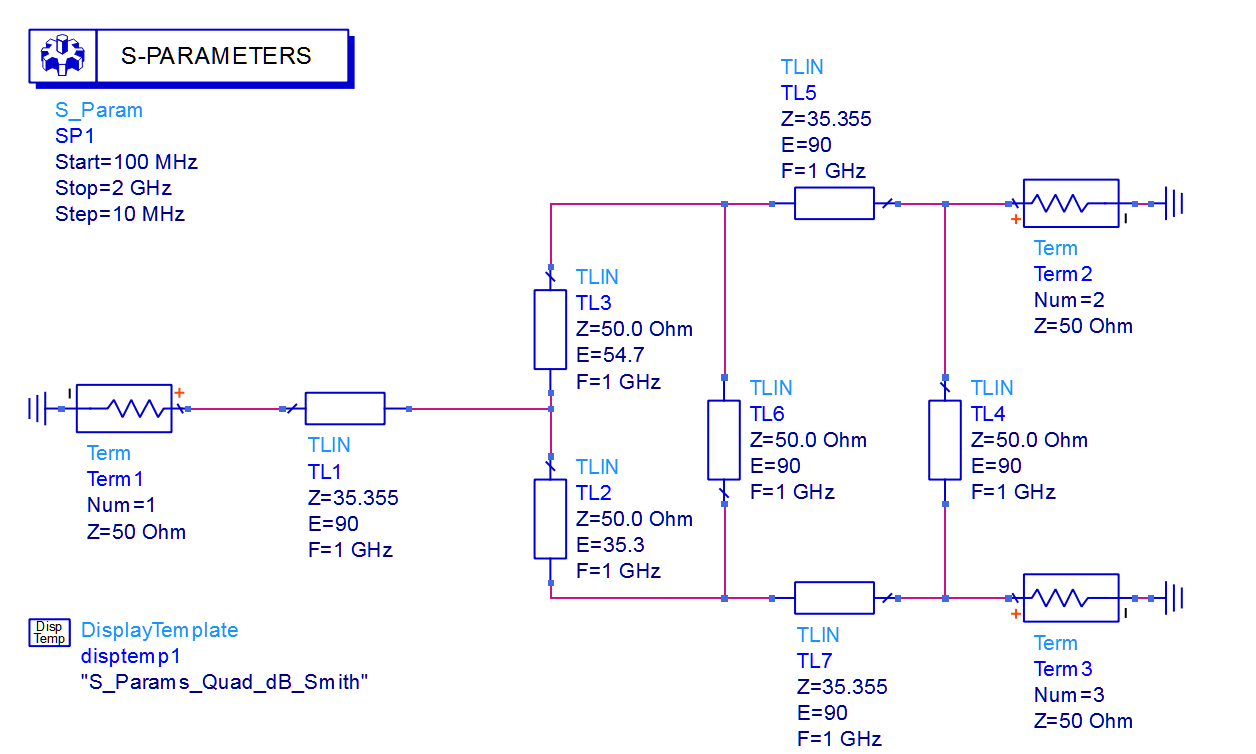
\includegraphics[width=0.8\linewidth]{img/Problem3/PowerSplitterSchematic.PNG}
    \caption{Schematic of the Designed Power Splitter}
    \label{fig:img/Problem3/PowerSplitterSchematic.PNG}
\end{figure}

\begin{figure}[H]
    \centering
    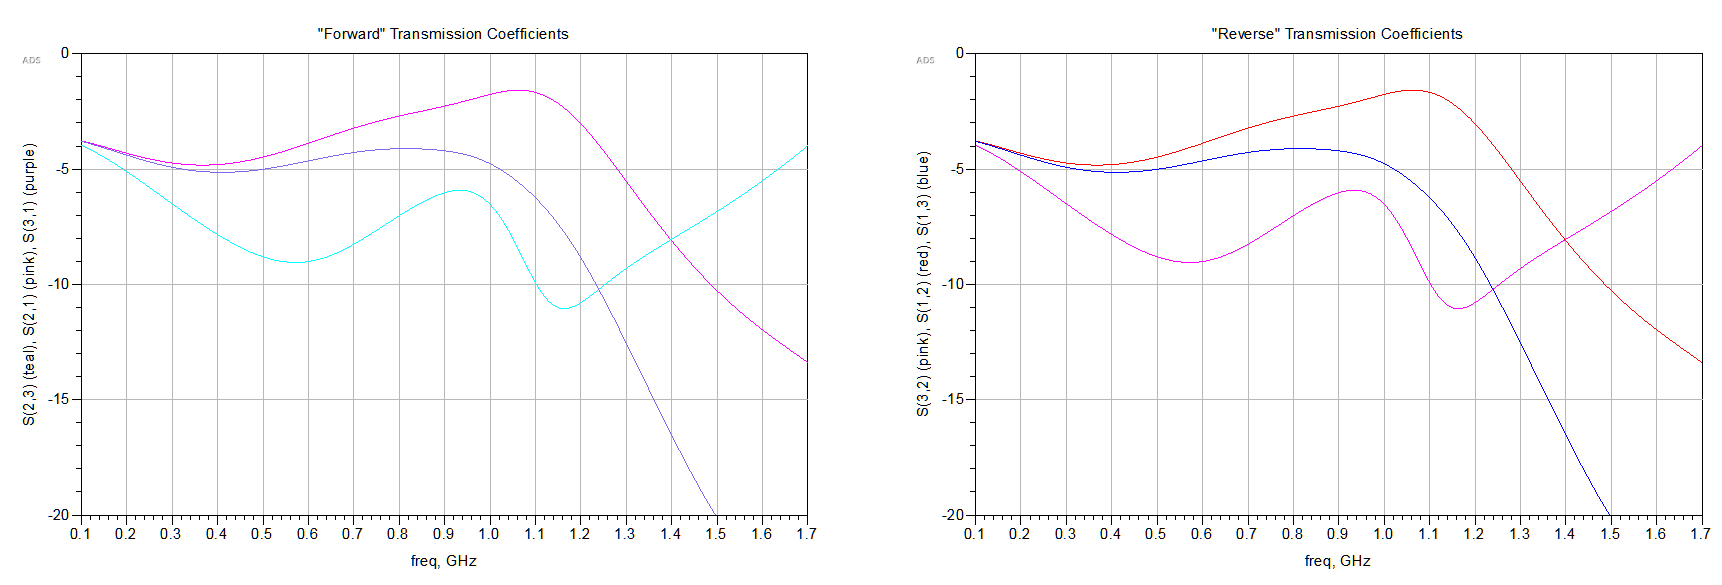
\includegraphics[width=0.8\linewidth]{img/Problem3/PowerSplitterTransmissionCoefficients.PNG}
    \caption{Transmission Coefficients for the Designed Power Splitter}
    \label{fig:img/Problem3/PowerSplitterTransmissionCoefficients}
\end{figure}

\begin{figure}[H]
    \centering
    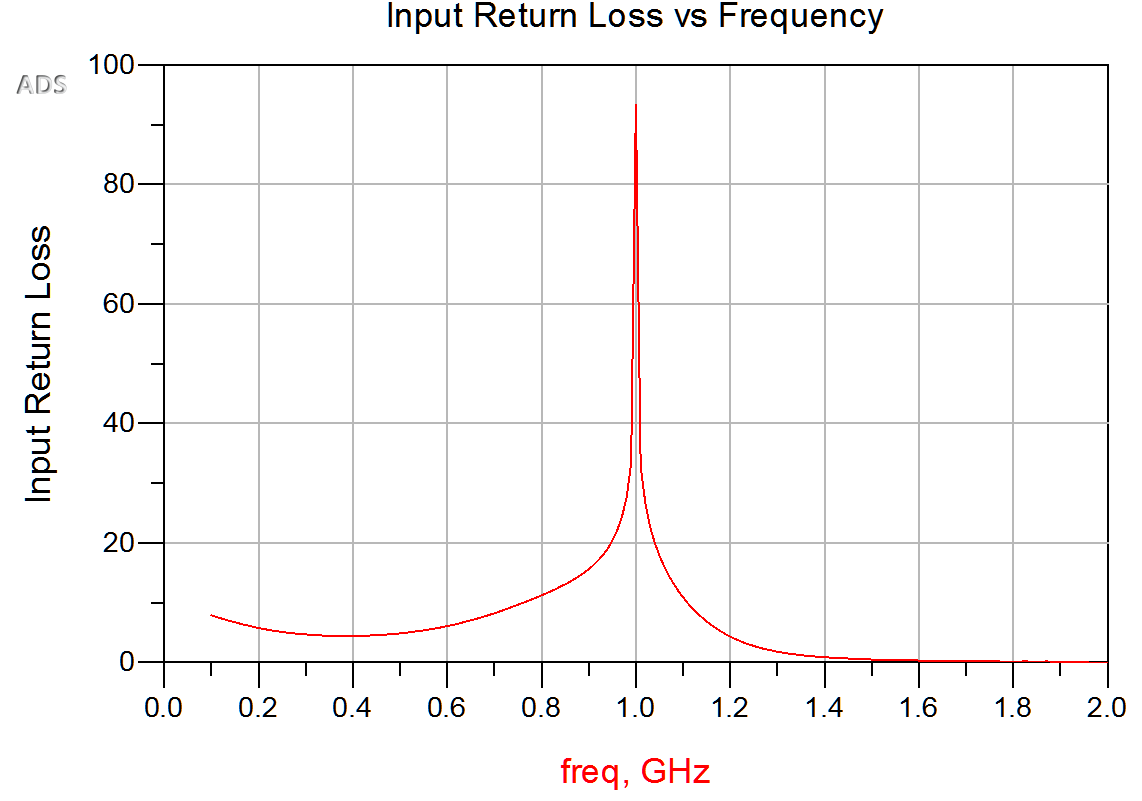
\includegraphics[width=0.8\linewidth]{img/Problem3/PowerSplitterInputReturnLoss.PNG}
    \caption{Input Return Loss for the Designed Power Splitter}
    \label{fig:img/Problem3/PowerSplitterInputReturnLoss.PNG}
\end{figure}
